\chapter{Logical Formalism and the Category of Categorizable Logics}

\section{Sequent Calculi as Canonical Presentations}

\subsection{The Sequent Form}

A \textbf{sequent} has the form:
\[ \Gamma \vdash \Delta \]
where:
\begin{itemize}
\item $\Gamma$ (antecedent) is a multiset of formulas (hypotheses)
\item $\vdash$ (turnstile) separates hypotheses from conclusions
\item $\Delta$ (succedent) is a multiset of formulas (conclusions)
\end{itemize}

Semantically: ``From the hypotheses $\Gamma$, at least one formula in $\Delta$ follows.''

\subsection{Why Sequent Calculi Are Canonical}

This work adopts sequent calculi as the canonical presentation for formal logics because:

\begin{enumerate}
\item \textbf{Structural transparency}: Antecedent/succedent restrictions are explicit in the syntax
\item \textbf{Cut elimination}: The fundamental meta-theorem of proof theory is directly expressible
\item \textbf{Definitional clarity}: Logical structure emerges from sequent restrictions and structural rules
\item \textbf{Structural rules are first-class}: Exchange, weakening, contraction are visible as inference rules
\item \textbf{Computational interpretation}: Sequent calculus proofs correspond naturally to programs (via Curry-Howard)
\end{enumerate}

Other presentations exist (natural deduction, tableaux, Hilbert systems) and are valid. They are isomorphic to sequent presentations for most logics. We choose sequent calculi for their \emph{structural explicitness}.

\subsection{Canonical Examples}

\subsubsection{LK: Classical Logic (Gentzen, 1935)}

\textbf{Sequent form}: $\Gamma \vdash \Delta$ (both unrestricted)

\textbf{Structural rules}: All present (Exchange, Weakening, Contraction on both sides)

\textbf{Logical characteristics}:
\begin{itemize}
\item Law of Excluded Middle (LEM): $\vdash A \vee \neg A$
\item Law of Non-Contradiction (LNC): $A \wedge \neg A \vdash$
\item Double negation elimination: $\neg \neg A \vdash A$
\item Explosion (ex falso quodlibet): $\bot \vdash Q$
\end{itemize}

\subsubsection{LJ: Intuitionistic Logic (Gentzen, 1935)}

\textbf{Sequent form}: $\Gamma \vdash A$ (restricted succedent: single formula or empty)

\textbf{Structural rules}: All present on antecedent; succedent restrictions make right-side structural rules moot

\textbf{Logical characteristics}:
\begin{itemize}
\item LEM is \emph{not} provable: $\not\vdash A \vee \neg A$
\item LNC remains: $A \wedge \neg A \vdash$
\item Double negation elimination fails: $\neg \neg A \not\vdash A$
\item Explosion remains: $\bot \vdash Q$
\item Constructive: proofs require explicit witnesses
\end{itemize}

\subsubsection{LDJ: Dual-Intuitionistic Logic (Urbas, 1996)}

\textbf{Sequent form}: $A \vdash \Delta$ (restricted antecedent: single formula or empty)

\textbf{Structural rules}: All present on succedent; antecedent restrictions make left-side structural rules moot

\textbf{Logical characteristics}:
\begin{itemize}
\item LEM remains: $\vdash A \vee \neg A$
\item LNC is \emph{not} provable (symmetric dual to LJ's failure of LEM)
\item Dual to intuitionistic logic: refutation calculus rather than proof calculus
\item Co-constructive: refutations require explicit counter-witnesses
\end{itemize}

\textbf{Distinction}: LDJ (proof calculus for dual-intuitionistic logic) differs conceptually from co-intuitionistic logic (refutation calculus). Both are related to ``dual-intuitionistic'' semantics but represent different formal systems.

\subsubsection{Monotonic Logic}

\textbf{Sequent form}: $A \vdash B$ (both restricted: single formula on each side)

\textbf{Structural rules}: Varies by family; typically full structural

\textbf{Logical characteristics}:
\begin{itemize}
\item Neither LEM nor LNC is provable
\item Negation and implication are inexpressible (not eliminated by axioms, but structurally unusable)
\item Only positive lattice operations: $\{\wedge, \vee, \bot, \top\}$
\item Formal intersection of LJ and LDJ restrictions
\end{itemize}

\section{The Two-Dimensional Lattice Structure}

\subsection{Horizontal Dimension: Antecedent/Succedent Restrictions}

For a fixed set of structural rules, logics vary by sequent restrictions. This forms a \textbf{horizontal diamond}:

\begin{center}
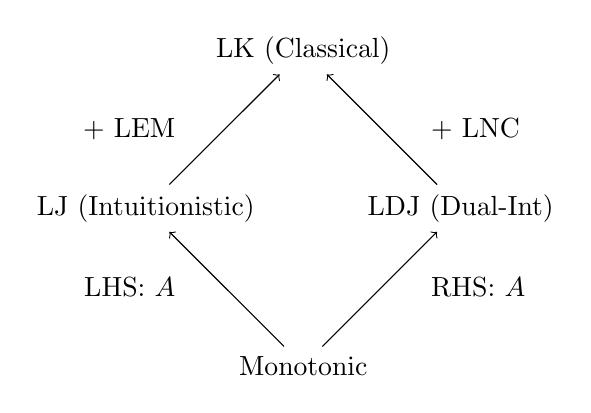
\begin{tikzpicture}[node distance=3cm]
\node (LK) at (0,2) {LK (Classical)};
\node (LJ) at (-2,0) {LJ (Intuitionistic)};
\node (LDJ) at (2,0) {LDJ (Dual-Int)};
\node (LM) at (0,-2) {Monotonic};

\draw[->] (LM) -- (LJ);
\draw[->] (LM) -- (LDJ);
\draw[->] (LJ) -- (LK);
\draw[->] (LDJ) -- (LK);

\node at (-1.5,1) [left] {$+$ LEM};
\node at (1.5,1) [right] {$+$ LNC};
\node at (-1.5,-1) [left] {LHS: $A$};
\node at (1.5,-1) [right] {RHS: $A$};
\end{tikzpicture}
\end{center}

\textbf{Interpretation}:
\begin{itemize}
\item \textbf{Top}: LK (no restrictions) → full classical power
\item \textbf{Left}: LJ (restricted RHS) → no LEM (constructive proofs)
\item \textbf{Right}: LDJ (restricted LHS) → no LNC (co-constructive refutations)
\item \textbf{Bottom}: Monotonic (both restricted) → neither LEM nor LNC
\end{itemize}

This diamond is parametrized by \{LEM, LNC\}. Every horizontal diamond in the category has this structure, regardless of structural rule configuration.

\subsection{Vertical Dimension: Structural Rule Presence/Absence}

Structural rules:
\begin{itemize}
\item \textbf{Exchange (E)}: Order of premises is irrelevant
  \[ \frac{\Gamma, A, B, \Delta \vdash \Theta}{\Gamma, B, A, \Delta \vdash \Theta} \]
\item \textbf{Weakening Left ($W_L$)}: Add hypotheses freely
  \[ \frac{\Gamma \vdash \Delta}{\Gamma, A \vdash \Delta} \]
\item \textbf{Weakening Right ($W_R$)}: Add conclusions freely
  \[ \frac{\Gamma \vdash \Delta}{\Gamma \vdash A, \Delta} \]
\item \textbf{Contraction Left ($C_L$)}: Merge duplicate hypotheses
  \[ \frac{\Gamma, A, A \vdash \Delta}{\Gamma, A \vdash \Delta} \]
\item \textbf{Contraction Right ($C_R$)}: Merge duplicate conclusions
  \[ \frac{\Gamma \vdash A, A, \Delta}{\Gamma \vdash A, \Delta} \]
\end{itemize}

Five binary parameters: $(E, W_L, W_R, C_L, C_R) \in \{0,1\}^5 \Rightarrow 2^5 = 32$ theoretical combinations.

\textbf{Meaningful clusters} (logical families):
\begin{itemize}
\item \textbf{Full Structural}: $E=1, W_L=1, W_R=1, C_L=1, C_R=1$ (classical family)
\item \textbf{Affine}: $E=1, W_L=1, W_R=1, C_L=0, C_R=0$ (allows erasure, no cloning)
\item \textbf{Relevant}: $E=1, W_L=0, W_R=0, C_L=1, C_R=1$ (allows cloning, no erasure)
\item \textbf{Linear}: $E=1, W_L=0, W_R=0, C_L=0, C_R=0$ (quantum-safe core)
\item \textbf{Order Calculi}: $E=0$ (order matters; various W/C configurations)
\item \textbf{Non-Structural}: $E=0, W_L=0, W_R=0, C_L=0, C_R=0$ (maximally resource-constrained)
\end{itemize}

\textbf{Vertical arrows}: Extension morphisms respecting structural rule containment. Example:
\[ \text{Linear} \to \text{Affine} \quad (\text{add } W_L, W_R) \]
\[ \text{Linear} \to \text{Relevant} \quad (\text{add } C_L, C_R) \]
\[ \text{Affine}, \text{Relevant} \to \text{Full Structural} \quad (\text{add remaining rules}) \]

\subsection{The Full Category: A Lattice of Lattices}

The complete structure:
\begin{itemize}
\item \textbf{Objects}: Logics $L = (\text{StructuralConfig}, \text{LHS-Restriction}, \text{RHS-Restriction})$
\item \textbf{Morphisms}: Extension or interpretability relationships respecting both dimensions
\item \textbf{Horizontal planes}: Each structural configuration forms a diamond (LK, LJ, LDJ, Monotonic)
\item \textbf{Vertical hierarchy}: Structural rule containment (Non-structural $\to$ Linear $\to$ Affine/Relevant $\to$ Full Structural)
\item \textbf{Commutative diagrams}: Both 2D (within diamonds) and 3D (across families)
\end{itemize}

\textbf{Example vertical tower}:
\begin{center}
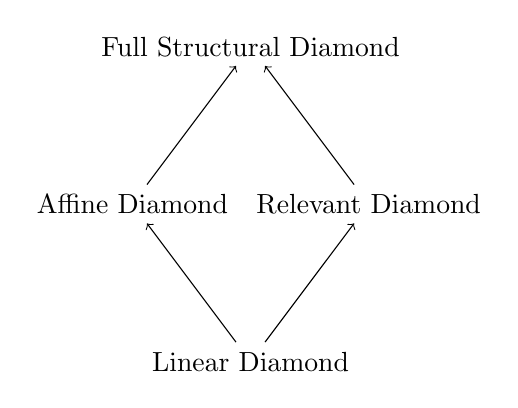
\begin{tikzpicture}[node distance=2cm]
\node (FS) at (0,4) {Full Structural Diamond};
\node (Aff) at (-1.5,2) {Affine Diamond};
\node (Rel) at (1.5,2) {Relevant Diamond};
\node (Lin) at (0,0) {Linear Diamond};

\draw[->] (Lin) -- (Aff);
\draw[->] (Lin) -- (Rel);
\draw[->] (Aff) -- (FS);
\draw[->] (Rel) -- (FS);
\end{tikzpicture}
\end{center}

Each ``diamond'' is itself a four-object commutative diagram (LK-variant, LJ-variant, LDJ-variant, Monotonic-variant for that structural configuration).

\section{The Logical Signature of Categorizable Logics}

A logic $L$ is \textbf{categorizable} if it admits a formal specification in terms of:

\subsection{Primitive Elements}

\begin{enumerate}
\item \textbf{Structural Rules}: Binary parameters $(E, W_L, W_R, C_L, C_R) \in \{0,1\}^5$
\item \textbf{Sequent Restrictions}: Binary flags (restricted\_LHS, restricted\_RHS) $\in \{0,1\}^2$
\item \textbf{Logical Connectives}: Subset of $\{\wedge, \vee, \neg, \to, \leftrightarrow, \bot, \top\}$ determined by restrictions
\item \textbf{Quantifiers} (if first-order): $\forall, \exists$ (possibly restricted)
\end{enumerate}

\subsection{Meta-Predicates}

\begin{itemize}
\item $\text{categorizable}(L)$: $L$ satisfies category axioms
\item $\text{morphism}(L_1, L_2)$: Formal extension or interpretability relation
\item $\text{diamond\_commutes}(D)$: $D$ is a commutative diagram
\item $\text{physical\_realizable}(L)$: $L$ embodies quantum symmetries
\end{itemize}

\subsection{Formal Axioms and Constraints}

\subsubsection{Category Axioms}

\textbf{Axiom 1 (Composition)}: If $f: L_1 \to L_2$ and $g: L_2 \to L_3$, then $(g \circ f): L_1 \to L_3$ exists and composition is associative.

\textbf{Axiom 2 (Identity)}: For every logic $L$, there exists $\text{id}_L: L \to L$ such that $f \circ \text{id}_L = f$ and $\text{id}_L \circ f = f$ for all applicable morphisms $f$.

\subsubsection{Logical Axioms (Provability Within Logics)}

\textbf{Axiom 3 (Explosion)}: $\bot \to Q$ is provable iff at least one of $\{W_L, W_R\}$ is present.

\emph{Proof sketch}: Weakening allows adding arbitrary formulas to sequents, enabling derivation from falsehood. Without weakening, $\bot$ is isolated and non-explosive.

\textbf{Axiom 4 (Law of Excluded Middle)}: $P \vee \neg P$ is provable iff succedent is unrestricted (RHS-Restriction = 0) and appropriate structural rules are present.

\emph{Intuition}: Multiple conclusions in the succedent enable classical disjunction proofs. Single-conclusion sequents (LJ, Monotonic) prohibit LEM.

\textbf{Axiom 5 (Law of Non-Contradiction)}: $\neg(P \wedge \neg P)$ is provable iff antecedent is unrestricted (LHS-Restriction = 0) and appropriate structural rules are present.

\emph{Intuition}: Symmetric dual to LEM. Single-hypothesis sequents (LDJ, Monotonic) prohibit LNC.

\subsubsection{Restriction-Restriction Axioms}

\textbf{Axiom 6 (Classical Completeness)}: If both LHS and RHS are unrestricted, and all structural rules are present, then all classical tautologies are derivable.

\textbf{Axiom 7 (Intuitionistic Fragment)}: If RHS is restricted and LHS unrestricted (with full structural rules), then LEM is not provable.

\textbf{Axiom 8 (Dual-Intuitionistic Fragment)}: If LHS is restricted and RHS unrestricted (with full structural rules), then LNC is not provable.

\textbf{Axiom 9 (Monotonic Intersection)}: If both LHS and RHS are restricted, then neither LEM nor LNC is provable, and negation/implication become structurally inexpressible.

\subsubsection{Structural-Logical Axioms}

\textbf{Axiom 10 (Weakening-Explosion)}: Weakening enables Explosion. Specifically, $\bot \to Q$ requires weakening to derive arbitrary conclusions from falsehood.

\textbf{Axiom 11 (Contraction-Classical)}: Contraction enables certain classical proof patterns. Without contraction, some classical theorems become unprovable.

\textbf{Axiom 12 (Exchange-Commutativity)}: Exchange enables premise commutativity. Without exchange, order matters (order calculi).

\subsubsection{Physical Realizability Axiom}

\textbf{Axiom 13 (Quantum-Safe)}: A logic $L$ is quantum-safe iff $W_L = 0$, $W_R = 0$, $C_L = 0$, $C_R = 0$.

\emph{Justification}:
\begin{itemize}
\item \textbf{No-cloning theorem}: Quantum states cannot be copied $\Rightarrow$ $C=0$ (no contraction)
\item \textbf{No-erasure theorem}: Quantum information cannot be destroyed $\Rightarrow$ $W=0$ (no weakening)
\end{itemize}

Non-structural logics ($E=0, W=0, C=0$) are maximally quantum-safe.

\section{The Theoretical Signature of the Category}

Meta-theorems governing relationships within the category.

\subsection{Fragment Relationships}

\textbf{Theorem 1 (Fragment Containment)}: If $L_1$ has more restrictions than $L_2$ (same structural rules), then $\text{theorems}(L_1) \subseteq \text{theorems}(L_2)$.

\emph{Example}: Intuitionistic theorems are a subset of classical theorems (LJ $\subset$ LK).

\textbf{Theorem 2 (Structural Extension)}: If $L_1$ has fewer structural rules than $L_2$ (same sequent restrictions), then $\text{theorems}(L_1) \subseteq \text{theorems}(L_2)$.

\emph{Example}: Linear logic theorems are a subset of affine logic theorems (LL $\subset$ ALL).

\subsection{Morphism Properties}

\textbf{Theorem 3 (Horizontal Morphisms)}: Morphisms within a horizontal diamond preserve structural rules and respect LEM/LNC relationships.

\textbf{Theorem 4 (Vertical Morphisms)}: Morphisms across families preserve sequent restrictions and respect structural rule containment.

\subsection{Diamond Properties}

\textbf{Theorem 5 (Diamond Commutativity)}: Every horizontal diamond is a commutative diagram. Paths from Monotonic to Classical (via LJ or LDJ) are equivalent.

\textbf{Theorem 6 (Greatest Lower Bound)}: Monotonic is the greatest lower bound (meet) of LJ and LDJ in each structural family.

\textbf{Theorem 7 (Least Upper Bound)}: Classical (LK-variant) is the least upper bound (join) of LJ-variant and LDJ-variant in each family.

\subsection{Vacancies (Future Formalization)}

The following are identified for future development:
\begin{itemize}
\item Formal proofs of Theorems 1--7
\item Complete specification of all morphisms between families
\item Natural transformations between logics
\item Categorical limits and colimits (products, coproducts, pullbacks, pushouts)
\item Decidability properties and their relationship to logical structure
\item Proof of functional incompleteness for non-classical logics
\end{itemize}

\section{Monotonic Logic as Formal Intersection}

\subsection{Structural Definition}

Monotonic logic is defined by the sequent form:
\[ A \vdash B \]
Both antecedent and succedent are restricted to single formulas.

\subsection{Formal Intersection of LJ and LDJ}

Monotonic logic is the \textbf{formal intersection} of intuitionistic and dual-intuitionistic restrictions:
\begin{itemize}
\item LJ: $\Gamma \vdash A$ (restricted RHS)
\item LDJ: $A \vdash \Delta$ (restricted LHS)
\item Intersection: $A \vdash B$ (both restricted)
\end{itemize}

\subsection{Loss of Negation and Implication}

Negation and implication are not eliminated by axioms---they become \textbf{structurally unusable}:
\begin{itemize}
\item Classical negation requires reasoning with full sequents (multiple hypotheses and conclusions)
\item Implication ($A \to B$) relies on sequent manipulations prohibited by double restrictions
\item Only positive lattice operations remain: $\{\wedge, \vee, \bot, \top\}$
\end{itemize}

This is a \textbf{structural limitation}, not an axiomatic one. The restricted sequent form makes negation and implication meaningless.

\subsection{Position in the Diamond}

Monotonic sits at the \textbf{bottom} of every horizontal diamond:
\begin{center}
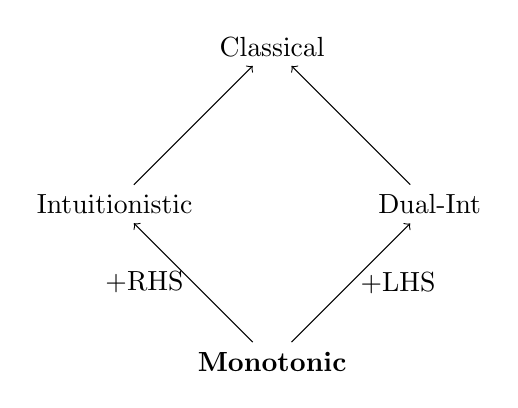
\begin{tikzpicture}[node distance=2.5cm]
\node (LK) at (0,2) {Classical};
\node (LJ) at (-2,0) {Intuitionistic};
\node (LDJ) at (2,0) {Dual-Int};
\node (Mon) at (0,-2) {\textbf{Monotonic}};

\draw[->] (Mon) -- (LJ) node[midway,left] {$+$RHS};
\draw[->] (Mon) -- (LDJ) node[midway,right] {$+$LHS};
\draw[->] (LJ) -- (LK);
\draw[->] (LDJ) -- (LK);
\end{tikzpicture}
\end{center}

\section{Physical Instantiation as Ground Truth}

\subsection{Logic $\to$ Computation Correspondence}

A categorizable logic paired with a theory instantiates as:
\begin{itemize}
\item \textbf{Software}: Executable program embodying logical structure
\item \textbf{Hardware}: Physical circuit (classical or quantum) implementing the logic
\end{itemize}

\textbf{Direct correspondences}:
\begin{center}
\begin{tabular}{l|l}
\textbf{Logic} & \textbf{Computational Paradigm} \\ \hline
Classical (LK) & Classical computation (unrestricted resource use) \\
Intuitionistic (LJ) & Constructive computation (explicit witnesses) \\
Linear (LL) & Resource-sensitive computation (single-use values) \\
Non-structural & Quantum computation or maximally constrained systems
\end{tabular}
\end{center}

\subsection{Physical Realizability Constraints}

Physical realizability is not metaphorical---it is a \textbf{hard constraint}:
\begin{itemize}
\item \textbf{No-cloning theorem} (Wootters \& Zurek, 1982): Arbitrary quantum states cannot be copied
  \[ \Rightarrow \text{Logics with } C=0 \text{ are quantum-realizable} \]
\item \textbf{No-erasure theorem} (Pati \& Braunstein, 2000): Quantum information cannot be destroyed without leaving a trace
  \[ \Rightarrow \text{Logics with } W=0 \text{ are quantum-safe} \]
\item \textbf{Non-structural logics}: $E=0, W=0, C=0$ respect both symmetries exactly
\end{itemize}

This connection is precise: structural rules in proof theory $\leftrightarrow$ resource management in computation $\leftrightarrow$ physical laws in quantum mechanics.

\subsection{Example: Linear Logic and Quantum Computing}

Linear logic (LL) with $W=0, C=0$ directly corresponds to quantum computation:
\begin{itemize}
\item No weakening: Information cannot be discarded (no-erasure)
\item No contraction: Values cannot be duplicated (no-cloning)
\item Exchange allowed: Order independence (when applicable)
\end{itemize}

This is not analogy---it is \textbf{structural isomorphism}. Linear logic is the natural logic for quantum-safe programming languages.

\section{Vacancies and Future Formalization}

The following are core structures requiring future development:

\begin{enumerate}
\item Formal proofs of all meta-theorems stated in Section 2.4
\item Complete specification of morphisms between all logical families
\item Detailed commutative diagrams for each horizontal diamond (32 potential families)
\item Full vertical hierarchy of all structural rule combinations
\item Natural transformations between logics (categorical structure)
\item Decidability properties and their relationship to logical structure
\item Proof of functional incompleteness claim for non-classical logics
\item Formalization of quantum realizability conditions (formal proofs)
\item Integration with Isabelle/AFP for mechanized verification (long-term)
\end{enumerate}

These vacancies are intentional: the abstract categorical structure is correct and complete at this stage. Details follow incrementally through future issues.
